\chapter{System Modeling}\label{chap::sysmodel}
This section outlines the approaches to modeling the thermodynamic and hydraulic behavior of the Decentralized Solution in the Cooltower. It begins with an overview of the overall structure of the model. Subsequently, the hydraulic and thermodynamic modeling of the individual components is discussed. 
% With particular attention given to the modeling of the valves. As unlike the other elements, the overflow mechanism (which is a valve) offers more flexibility within the optimization process, allowing exploration of alternative designs for further research. \todo{mss dit gewoon weghalen gezien ik dit meer ga toelichten in het optimalisatie hoofdstuk}
Afterwards, the peak and demand of the system are analyzed. Finally, a review of existing software tools for simulating district heating networks is presented. 

\section{Preliminaries}\label{sec::preliminaries}
Several general assumptions commonly used in the literature on  district heating networks and some dimesionless variables are outlined below. These assumptions are used throughout this chapter. Additional assumptions specific for particular methods are discussed in their dedicated sections.

This chapter focuses on modeling district heating networks. However, the same approach is applicable to district cooling systems, with modifications to account for the switch from heating to cooling.

\subsection{Modeling assumptions}
One of the most important modeling assumptions is that the hydraulic and thermodynamic systems can be assumed to be decoupled. It means that first the hydraulics calculation is completed, resulting in a mass flow, which is then used for the thermodynamics. The speed of sound in the water is (1481 m/s at 20 $^{\circ}\text{C}$ \cite{speedofsound}), causing the changes in flow rate and pressure to be within seconds in a small district heating network like a DCS. In contrast with the spread of thermodynamic changes as these travel at the speed of the maximum flow rate, which is around 3 m/s. This difference in time scale between the thermodynamics and hydraulics validates their decoupling \cite{KUNTUAROVA}.

Furthermore, these are the other assumptions applied in this chapter \cite{MAURER2021244,sibeijn2025economic,KUNTUAROVA,PipePDE}.
\begin{itemize}
    \item The water is incompressible, has a constant density and heat capacity. 
    \item Frictional heat is negligible.
    \item The fluid flow is turbulent and fully developed.
    \item The pipes are cylindrical and are fully filled with water.
    \item No water leaves the pipe system.
    \item The ambient temperature is constant along the length of the pipe.
    \item Homogeneous mixing at the pipe junctions.
    \item Thermal interaction between the supply and return pipes is not included.
    \item The total thermal resistance per unit length of pipe is constant.
    \item The diffusion of heat in the axial direction is neglected. 
\end{itemize}

% It is assumed that the hydraulics are in a steady state due to the high speed of sound in water (1481 m/s at 20 $^{\circ}\text{C}$ \cite{speedofsound}) causing the changes in flow rate and pressure to be within seconds in a small district heating network like a DCS. Whereas, the thermodynamic changes spread at a much lower speed with a maximum flow rate of around 3 m/s. Furthermore, it is assumed that the water is incompressible, has a constant density and heat capacity, and that frictional heat is negligible. Based on these assumptions, the hydraulic and thermodynamic systems can be assumed to be decoupled. In addition, it is assumed that the pipelines are cylindrical and completely filled with water. 

% Andere aannames die mogelijk hier hier nog kunnen worden benoemd afhankelijk van hoe het gaat met de methods voor de pijpleiding:
% - zelfde diameter van de pijpleiding?
% - constant heat transmission coefficient
% - ambient temperature constant along the length of the pipeline
% - spatially homogenous velocity and temperature in the cross-seciton
% - heat diffusion in axial direction is neglected
% deze hierboven komen allemaal van Maurer.
% - turbulente flow? [Yvo Putter] -> Dit goed checken, moet ook turbulent flow aannemen voor de darcy weisbach
% - fully developed? [Yvo]
% - homogeneous mixing at pipe junctions
% - one directional flow?
\subsection{Dimensionless Numbers}
\textbf{The Reynolds Number (Re)} is the primary parameter correlating the viscous behavior of all Newtonian fluids \cite{white2011fluid}. It is a ratio between the internal and viscous forces within a fluid. And it is used as an indicator for a flow to be laminar or turbulent. 

\begin{equation}\label{eq::Re}
R e=\frac{\rho D v}{\mu}=\frac{4 \dot{m}}{\pi D \mu}
\end{equation}

Where $\rho$ [kg / m$^3$] is the density of the fluid, $v$ [m/s] the fluid velocity and $D$ [m] the diameter of the pipe, $\mu$ its dynamic viscosity [kg / (m s)] and $\dot{m}$ [kg/s] is the mass flow. 

\textbf{The Darcy friction factor (f)} can be found in the Darcy-Weisbach equation, which calculates the pressure flow drop through a pipe using the pipe flow. The coefficient can be determined using the Moody diagram, where $f$ is plotted against the Reynolds number for different relative roughnesses $\epsilon / d$. It can also be determined analytically using the Colebrook-White equation \ref{eq:CoolbrookWhite}, which is the most popular method, for the transition region (2300 $\leq$ Re $\leq$ 4000) and the turbulent region (Re $\geq$ 4000) in smooth and rough pipes \cite{Darcyfrictionfactor}. This requires an iterative approach to determine $f$. There are also non-iterative methods, but they have a relative error to the Colebrook-White Equation. Nonetheless, the authors of \cite{Darcyfrictionfactor} found that for certain correlations the error is negligible.

\begin{equation}\label{eq:CoolbrookWhite}
\frac{1}{\sqrt{f}}=-2 \log \left(\frac{\epsilon}{3.7 D}+\frac{2.51}{\operatorname{Re} \sqrt{f}}\right)
\end{equation}

With the roughness of the pipe $\epsilon$ [m].

\textbf{The Courant number (C)} can be interpreted as the distance of the advective flow per element in the space domain. It is used in the Courant–Friedrichs–Lewy (CFL) condition, which is a necessary condition to guarantee numerical stability when solving partial differential equations with an explicit approach. In the 1-dimensional case, it is defined as
\begin{equation}
    C = \frac{v \Delta t}{\Delta x} \leq 1
\end{equation}
With $v$ [m/s] as the propagation speed, $\Delta t$ [s] the simulation timestep, and $\Delta x$ [m] the discrete spatial interval \cite{MaxCourant}. 

\section{Model structure}
This section discusses multiple approaches suitable for the overall structure of the model and various modeling methods for the thermodynamics and hydraulics found in district heating networks. In general, three different modeling techniques can be distinguished for any type of system

\begin{itemize}
    \item \textbf{White-box} modeling looks at physical laws and parameters to create a model. It is the more conventional option used in the majority of the DHN modeling articles \cite{sibeijn2025economic,PipePDE}.
    \item \textbf{Black-box} modeling puts the behavior of the entire system into one function, which is determined using data-driven methods. In \cite{GUELPA2016586}\cite{KECEBAS2012339}, it is applied to district heating networks.
    \item \textbf{Grey box} modeling is a combination of the two above and can be found in a DHN context in \cite{grey1}\cite{grey2}. 
\end{itemize}
This literature survey focuses on the white box model, as a more thorough understanding of the system's inner workings is preferred. 

District heating networks are branched or looped-based networks, making them perfectly suited for modeling with a graph approach. The graph consists of nodes, which are junctions in the system, connected by edges. An edge is a pipe, potentially equipped with a heat exchanger, pump, or valve \cite{sibeijn2025economic}. On the edges, producers can add heat, and consumers can subtract it. The temperature at each node is determined by a weighted average of the incoming mass flows and their respective temperatures. All outgoing edges from the node are assigned the same temperature as the node itself. To calculate the mass flows and pressure within the network, Kirchhoff's two laws must be upheld. The first law asserts that the total mass flow entering and leaving a node must be equal, ensuring mass conservation. The second law requires that the net pressure drop around any closed loop in the network must be zero, maintaining pressure balance. The pressure loss within the pipes depends quadratically on the flow, making the hydraulics a system of non-linear equations. As we assume a decoupled system, the hydraulic problem is computed first, after which the obtained mass flow rates are used for the thermodynamic system. 

To solve this hydraulic system of non-linear equations, we assume that the demand and heat supply are known, leaving the pipe flows to be determined. This can be done by making use of iterative methods like Hardy-Cross \cite{HardyCross} and Newton-Raphson \cite{NewtonenHard}. These methods make an initial guess of the flow and then iteratively adjust this guess until it converges. Where the Hardy-Cross method runs through each loop independently, the Newton–Raphson method runs through all loops simultaneously \cite{NewtonenHard}. In \cite{STEVANOVIC}, the authors claim that they developed a method of square roots for solving the linearized system that outperforms the Hardy-Cross method in convergence time and validated it with real data. Also the aggregated models from \cite{LARSEN2002995} (also tested with real data) converge quicker (which is mainly interesting for big district heating networks) and overcome some of the limitations of the Hardy-Cross method. Where Arsene et al. \cite{ARSENE} found that for low flow rates the Newton-Raphson and Hardy-Cross methods experienced weak convergence and propose a new method which is a combination of the Newton-Raphson method and a loop corrective method. 

The thermodynamic behavior of the edge in the system is described by a PDE. Different solutions for this equation are discussed in more detail in Section \ref{sec::thermo}

\section{Hydraulic modeling}\label{sec::hydromodel}
It is essential to know the pressure loss across all components, as this information, combined with Kirchhoff's laws, enables the determination of fluid flow throughout the district heating network. 

The total pressure loss of a pipe system can be divided into major and minor losses. The major pressure loss ($\Delta p_p$) is caused by friction along the length of the pipe and the height difference, the minor losses ($\Delta p_m$) are the result of the entrance or exit of the pipe, fittings, bends, valves, and sudden expansions and contractions of the pipes. Although they are called minor losses, a partially closed valve can cause a greater pressure loss than a long pipe \cite{white2011fluid}. Adding the heat exchangers ($\Delta p_{hex}$) to the major losses in this pipe system results in the following definition of total pressure change within a loop of the system. 

\begin{equation}
    \Delta p_{\text{tot}} = \sum \Delta p_{p} + \Delta p_m + \sum \Delta p_{\text{hex}} 
\end{equation}
The pressure loss over the pipes is discussed in Section \ref{sec::hydropipes}. Where $p_m$ depends on the type and size of the heat exchanger \cite{YvoPutter}, which needs to be determined for the DCS of the Cooltower. The minor losses are defined according to Equation \ref{eq::minorpres}.

\begin{equation}\label{eq::minorpres}
    \Delta p_m = \frac{\rho_w v^2}{2g} \sum \zeta
\end{equation}

The fluid velocity $V$ [m/s], the density of water $\rho_w$ [kg/m$^3$], the loss coefficient $\zeta$ [-], and $g$ the gravitational acceleration [m/s$^2$]. This formula holds that when all pipes have the same diameter, if the diameter changes, the fluid velocity will be affected. In that case, the losses need to be added separately. The manufacturer often provides the loss coefficients. However, the term is not based on the Reynolds Number or the roughness of the pipe, but solely on its diameter and assuming a turbulent flow \cite{white2011fluid}. If adding minor losses for a large pipe system becomes too cumbersome, one might choose to apply an additional percentage (5 to 20\%) on pipe friction losses \cite{echtephdthesis}. The pressure loss of the valves is discussed in more detail in Section \ref{sec::valves}.

%% ## HEAD
% In the literature, head (Equation \ref{eq::head}) is often used instead of pressure to describe hydraulic losses. 
% \begin{equation}\label{eq::head}
%     h = \frac{p}{\rho_w g}
% \end{equation}
% With head $h$ [m], pressure $p$ [Pa], gravitational constant $g$ [m/s$^2$], and the height to a certain reference point $z$ [m]. 

% The total head loss of a pipe system can be divided into major and minor losses. The major loss ($h_f$) is caused by the friction along the length of the pipe, the minor losses ($h_m$) are the result of the pipe entrance or exit, fittings, bends, expansions and contractions of the pipes and valves. Although they are called minor losses, a partially closed valve can cause a greater head loss than a long pipe \cite{white2011fluid}. Adding the heat exchangers ($h_{hex}$ to the major losses in this pipe system results in the following definition of the total head. 
% \begin{equation}
%     \Delta h_{tot} = h_f + \sum h_m + h_{hex} 
% \end{equation}
% The friction head loss $h_f$ is discussed in Section \ref{sec::hydropipes}. Where $h_m$ depends on the type and size of the heat exchanger \cite{YvoPutter}, which needs to be determined for the DCS of the Cooltower. The minor losses are defined according to Equation \ref{eq::minorhead}.

% \begin{equation}\label{eq::minorhead}
%     \sum h_m = \frac{V^2}{2g} \sum K
% \end{equation}

% The fluid velocity $V$ [m/s] and the loss coefficient $K$ [-]. This formula holds when all the pipes have the same diameter, as if the diameter changes, it affects the fluid velocity. In that case the losses need to be added separately. The loss coefficient is often provided by the manufacturer. However, the term is not based on the Reynolds Number or the roughness of the pipe, but solely on its diameter and assuming a turbulent flow \cite{white2011fluid}. The head loss of the valves is discussed in more detail in Section \ref{sec::valves} to further discover the modeling possibilities for the overflow mechanism. 


\subsection{Pipes}\label{sec::hydropipes}
An approximation of the 1-dimensional compressible Euler equations for cylindrical pipes is used to describe the dynamics within a pipe \cite{Krug2020}. The first two equations, the continuity equation and the 1D momentum equation, are needed for the calculation of the mass flows. They are stated down below.

\begin{equation}
\partial_t \rho_w+\partial_x\left(\rho_w v\right)=0
\end{equation}
\begin{equation}
\partial_t (\rho_w v)+\partial_x(\rho_w v^2)+ \partial_x p+\rho_w g \hat{z}  +f \frac{\rho_w}{2 D}|v| v=0
\end{equation}
Where the pressure in the pipe $p$ [Pa], the slope of the pipe $\hat{z}$ [-] and friction coefficient $f$ [-]. Given the substantial difference in time scales between the hydraulics and thermodynamics, and the dominant influence of the friction term over the inertial term, the hydraulic system can be assumed to be in a steady state. In combination with the the assumptions stated in Section \ref{sec::preliminaries}, the following holds: $\partial_x v = 0, \partial_t \rho_w = 0$, $\partial_x \rho_w = 0$ and $\partial_t v = 0$. Making the continuity equation obsolete and results in the approximation of the momentum equation below \cite{sibeijn2025economic}. 
\begin{equation}\label{eq::mom}
\partial_x p + \rho_w g \hat{z} +f \frac{\rho_w}{2 D}\left|v\right| v=0
\end{equation}
Substituting $v = \frac{4 \dot{q}}{\pi D^2}$ into \eqref{eq::mom} and discretizing $\partial_x p = \frac{\Delta p}{L}$ leads to:
\begin{equation}
    \Delta p = p_{p} =  f \frac{8\rho_w L}{\pi^2 D^5}\left|q\right| q + \rho_w g L \hat{z}
\end{equation}
With the flow rate $q$ [m$^3$/s] and the length of the pipe $L$ [m]. The first term on the right side of the equation is equal to the Darcy-Weisbach equation, which describes the pressure loss due to the friction of the fluid with the pipe wall.  

%% ###HEAD
% Rewriting the equation into the head loss gives:

% \begin{equation}
%     h_f = f \frac{8 L}{\pi^2 d^5 g}\left|q\right| q + \hat{z}
% \end{equation}


\subsection{Valves}\label{sec::valves}
Valves regulate the pressure or flow in a pipe system. The Cooltower's heat distribution system contains multiple different types of valves. The pressure losses due to the valves can be calculated in a slightly different manner than the general relation for minor pressure loss in Equation \ref{eq::minorpres}, stated in Equation \ref{eq::realminorpres}, giving a more precise definition for the valves \cite{Artikelphdchris}. 

\begin{equation}\label{eq::realminorpres}
    \Delta p_{v} = \left( \frac{\dot{V}}{K_v} \right)^{2} \frac{\rho}{\rho_{\text{ref}}}    
\end{equation}
With the hydraulic conductivity parameter $K_v$  [m$^3$/h/$\sqrt{bar}$], the volumetric flow rate $\dot{V}$ [m$^3$/h], the actual fluid density during simulations $\rho$ [kg/m$^3$], and the fluid density during the manufacturer's $K_v$ measurements $\rho_{ref}$ (typically 1000 kg/m$^3$). The calculation of the valve characteristic $K_v$, which varies with the valve's opening position, depends on the valve type. It is important to mention that for small valve lifts, the $K_v$ value cannot be determined accurately because it exceeds the required tolerances of the basic shape of the valve. The valve's control range is determined up to a 10 percent deviation of the basic shape. When it goes outside of this control range, the valve becomes unpredictable. The manufacturer provides the control range \cite{echtephdthesis}.

\subsubsection{2-Way Control Valves}
At first, we have the 2-way control valves focused on controlling the flow. When this valve is a basic linear 2-way valve, $K_v$ can be determined using \ref{eq::linear2valve}. Equation  \ref{eq::equalpercentvalve} applies to an equal percentage valve. Both equations are in accordance with the VDI/VDE2173 standard \cite{VDI/VDE2713}. 

\begin{equation}\label{eq::linear2valve}
    \frac{K_v}{K_{vs}} = \left( 1 -\frac{K_{v,0}}{K_{vs}} \right) \frac{h_{lift}}{h_{\infty}} + \frac{K_{v,0}}{K_{vs}}
\end{equation}
\begin{equation}\label{eq::equalpercentvalve}
    \frac{K_v}{K_{vs}} = {\left(\frac{K_{vs}}{K_{v,0}} \right)}^{\frac{h_{lift}}{h_{\infty}} - 1}
\end{equation}

With the $K_v$ value for the completely opened valve $K_{vs}$, the $K_v$ value at the points where the basic shape of the valve characteristic intersects with the y-axis $K_{v,0}$ and the dimensionless valve displacement $\frac{h_{lift}}{h_{\infty}}$ which ranges from 0 to 1 \cite{Artikelphdchris}. The differential pressure control valve is a specialized type of control valve designed to maintain a predefined pressure difference across a pipe. Unlike the previously discussed control valves, it directly controls the pressure drop over the pipe, not its flow. However, in practical applications, the valve is not ideal. The actual pressure difference across it may deviate from the setpoint. Especially for small valve lifts, the shape of the actual $K_v$ value cannot be accurately defined anymore. Therefore, $K_{vr}$ is defined as the minimum $K_v$ value for which the deviation from the reference curve remains within 10\% and the $h_{\text{lift}}$ associated with it is called $h^{*}$. Below this threshold, the valve operates outside its controllable range, and its behavior becomes unreliable. The modeling of such non-ideal behavior is further elaborated in \cite{echtephdthesis}. In case the valve is closed, the valve leakage $K_{\text{v,leak}}$ is defined.  

\begin{figure}[h!]
    \centering
    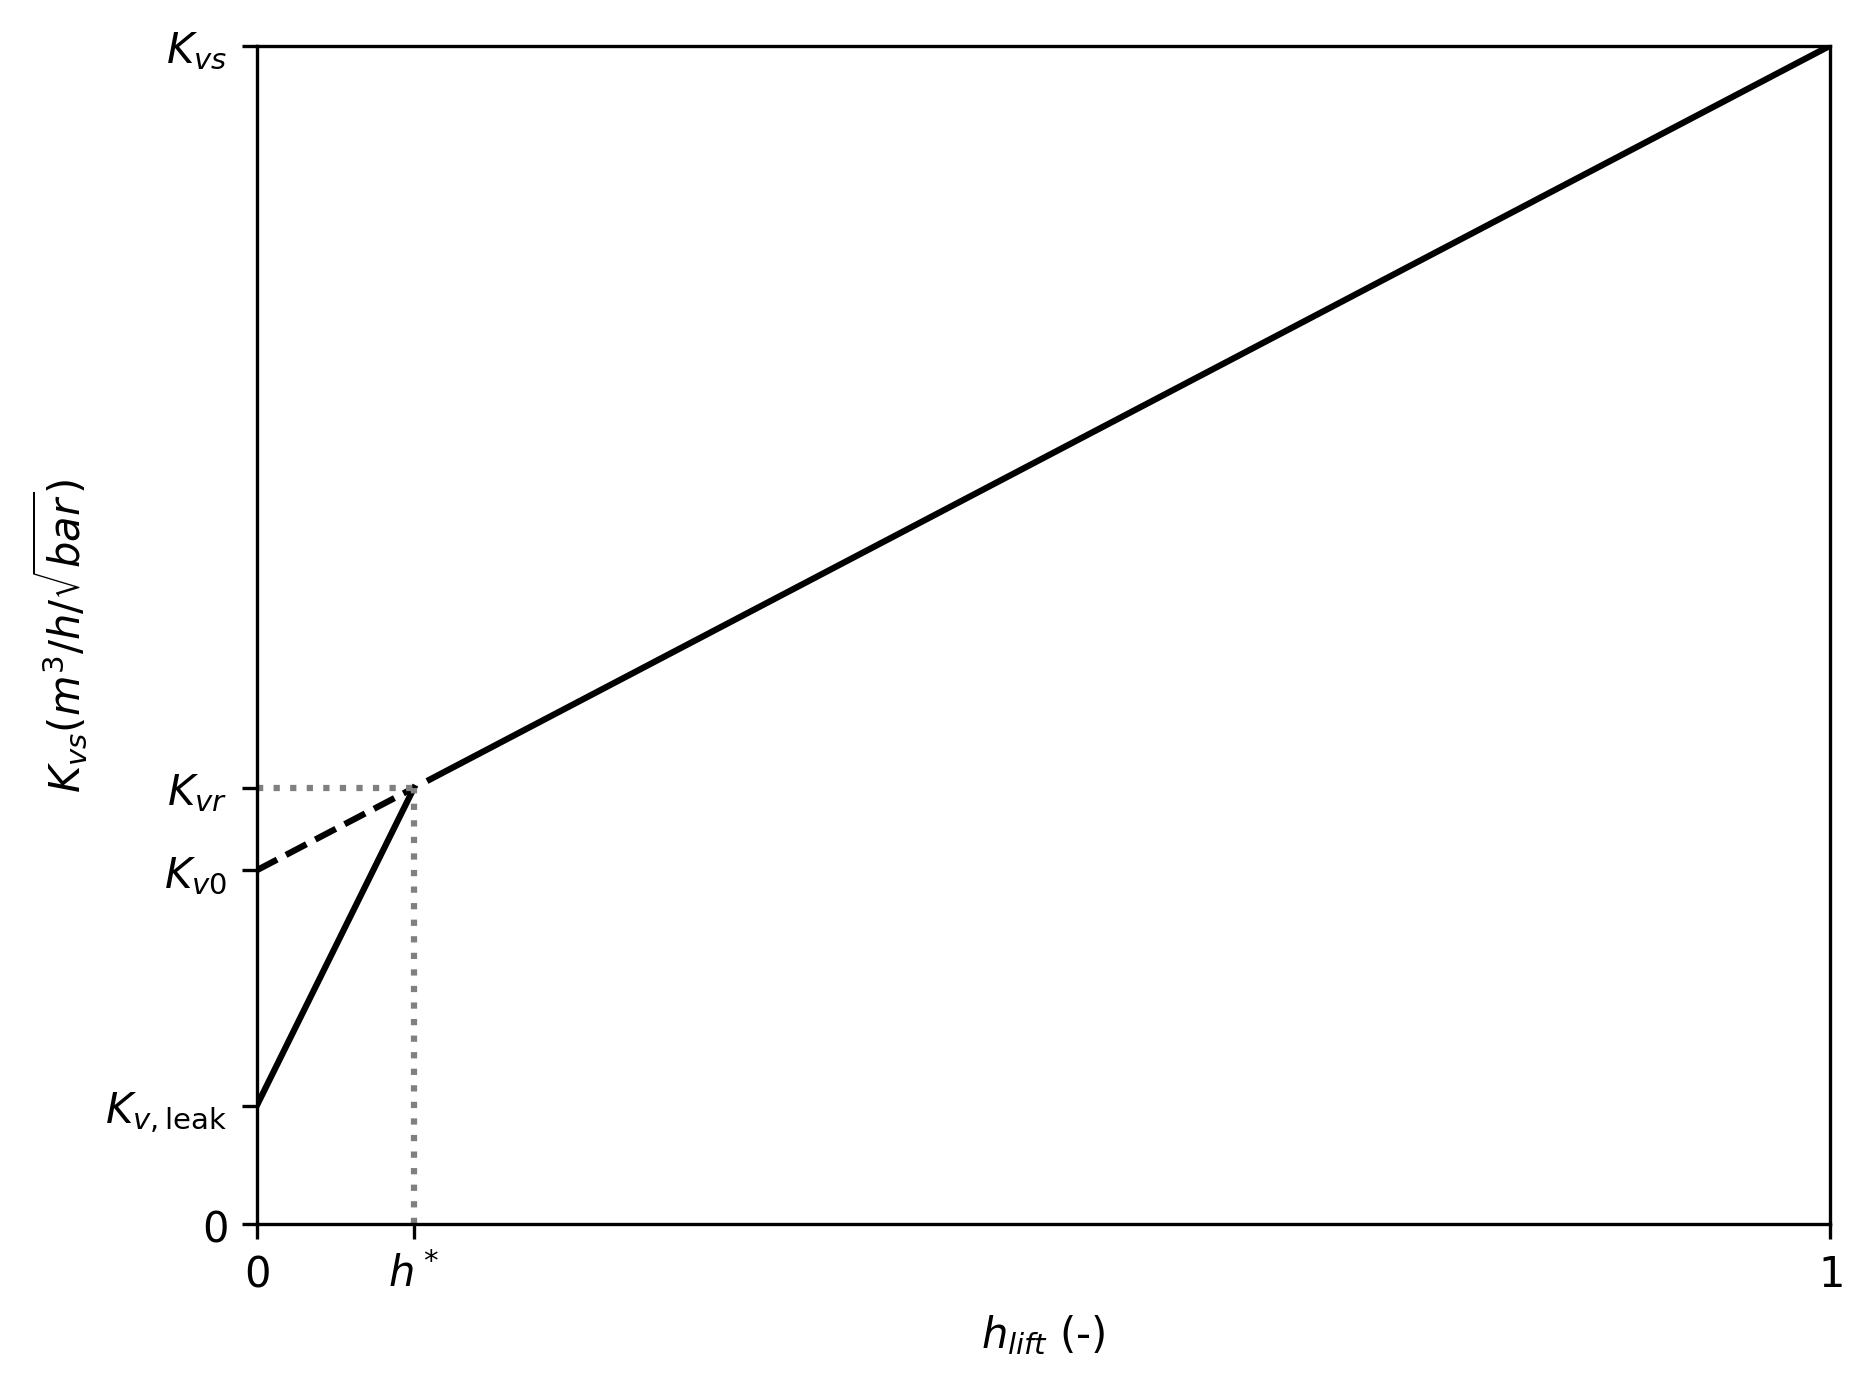
\includegraphics[width=0.65\linewidth]{Literature Survey - DCSC template/figuresLIT/Kvs_plot.png}
    \caption{The characteristic of a linear valve, below the valve lift of $h^*$ the control is unstable. It was assumed that the $K_v$ value is linear in the unstable region \cite{echtephdthesis}.}
    \label{fig:enter-label}
\end{figure}

\subsubsection{3-Way Control Valves}
There are also 3-way valves within the system. For these valves, the hydraulic resistance is defined over two valve entrance ports A and B.
The valve characteristic pair can be complementary. In the case, it is a 3-way linear valve port A can be described using Equation \ref{eq::linear2valve} and port B using Equation \ref{eq::3way-valve}. Respectively, changing the valve characteristic formula into Equation \ref{eq::equalpercentvalve} results in a 3-way equal percentage valve. However, sometimes the ports contain two different valve characteristics. 

\begin{equation}\label{eq::3way-valve}
    \frac{K_{v,B}}{K_{vs}} = 1 - \frac{K_{v,A}}{K_{vs}}
\end{equation}

The heat interface units present in the Cooltower, the Arctic WKW-S 4P \cite{fortes_wkw_s_4p}, contain a 6-way ball valve. This valve can be modeled as two interconnected 3-way valves with synchronized control logic. In this simplified model, each valve operates in a binary manner, either fully open or fully closed. Together, they determine whether the heat interface unit is in heating or cooling mode. Sometimes, the 6-way valve can also perform flow control, but not in our case. As this thesis focus solely on the heat distribution network, we can assume this valve to always stand in heating mode.


\subsubsection{Overflow Mechanism}
The overflow mechanisms of the Cooltower can be found on the top floor of each riser, where they are connected to the apartment's delivery set. When customers consume little or no heat, the flow rate of the water will decrease, causing the temperature within the supply network to decrease. In such a scenario, the overflow mechanisms' function is to maintain a high enough water temperature to still comply with water heat regulations. It performs this task by opening the valve, thereby increasing the flow rate. The overflow mechanism is a two-way flow control valve connected to a thermostat. 



\todo[inline]{Hier nog kort stukje over de precieze klep en het klep type na gesprek met Arjen en de setpoint temperatuur}
 
In addition to its current function, this thesis seeks to decrease the flow rate using the overflow mechanism to lower the eventual return temperature. The water stays longer in the distribution network and loses more heat to its surroundings. However, the original working of the overflow mechanism mainly increases the flow rate. With the optimization of the valve displacement of the overflow mechanism, we try to find the optimal trade-off between the opposing actions achieving both functions of the overflow mechanism. This will be further discussed in Section \ref{chap::optimization}.

% \todo[inline]{mogelijk nog overstorten benoemen?}
% \todo[inline]{Kan hier mogelijk nog wat zeggen over de square opening valve}
\subsection{Pumps}
Pumps supply the pressure necessary for the fluid to flow through the network. Centrifugal pumps are the most commonly used pumps in district heating networks. The pump is characterized by its performance curve, as shown in Figure \ref{fig::pumpcharacteristic}, which illustrates the relationship between pump head (or pressure) and the volumetric flow rate. This figure includes curves for various rotational shaft speeds. Also plotted is the system head curve, with the operating points of the system located at the intersections between the pump and system curves. The figure further includes iso-efficiency lines, which represent constant pump efficiency across different operating conditions. Changes in valve positions alter the system head curve, thereby shifting the operating point. Combining the position of the valves and the rotational speed of the shaft makes it possible to keep the pump operation efficient. Pump curves can be modeled using a polynomial law \cite{echtephdthesis}. 

\begin{equation}\label{eq::pumpchar}
    \Delta p_{p} = \sum^{\text{n}}_{\text{i=1}} \left( c_i(\omega)  \dot{V}^{i} \right)
\end{equation}

With the rotational shaft speed $\omega$ and the polynomial constants $c_i(\omega)$. 

\begin{figure}[h!]
    \centering
    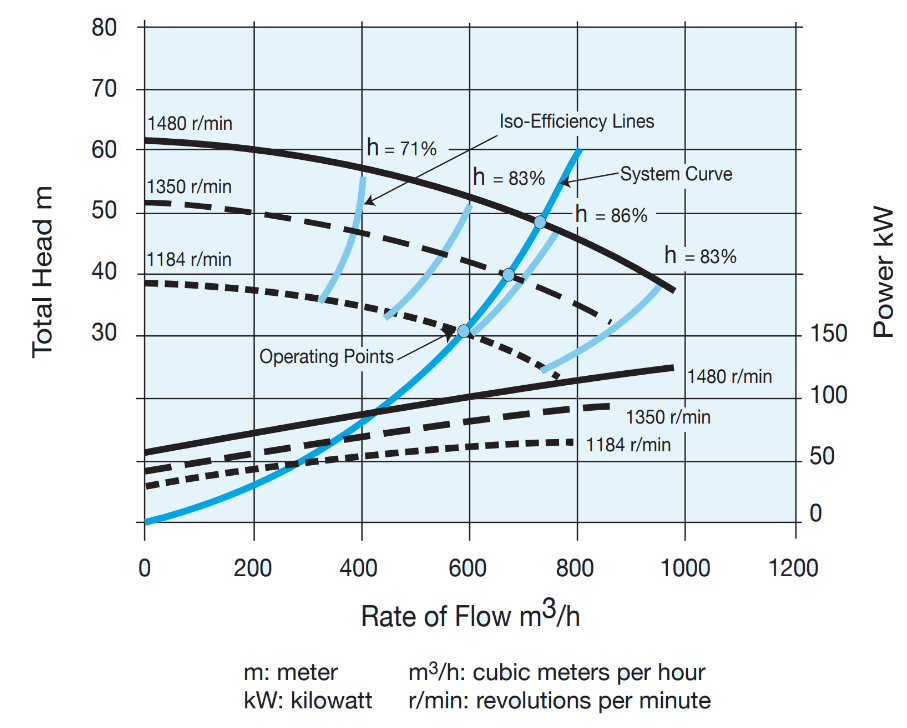
\includegraphics[width=0.6\linewidth]{Literature Survey - DCSC template/figuresLIT/pumpgoed.png}
    \caption{Pump characteristic head curves, containing iso-efficiency curves \cite{pumpcharacteristics}.}
    \label{fig::pumpcharacteristic}
\end{figure}

Variations in the operation of the pumps can be described using the affinity laws. These laws correlate changes in rotational shaft speed with changes in volumetric flow rate, head, and shaft power, assuming constant efficiency. 
\begin{equation}
\frac{\dot{V}_1}{\dot{V}_2}=\frac{\omega_1}{\omega_2} \quad \frac{H_1}{H_2}=\left(\frac{\omega_1}{\omega_2}\right)^2 \quad \frac{P_1}{P_2}=\left(\frac{\omega_1}{\omega_2}\right)^3
\end{equation}
For larger changes in the angular velocity of the shaft the affinity laws do not hold as parameters like the Reynolds number and friction change accordingly, influencing the efficiency of the pump. 
The pump's efficiency consists of three parts: volumetric ($\eta_v$), hydraulic ($\eta_h$), and mechanical ($\eta_m$), their relation is given by
\begin{equation}\label{eq::effpump}
    \eta = \eta_v\eta_h\eta_m
\end{equation}
Efficiency is in the following way related to the power delivered to the fluid ($P_w$).

\begin{equation}\label{eq::}
    \eta = \frac{P_w}{P_{in}} = \frac{\rho_w g \dot{V} H}{\omega T}
\end{equation}
With input power $P_{in}$ [W] and the shaft torque $T$ [N m] \cite{white2011fluid}. 

\section{Thermo-Dynamic modeling}\label{sec::thermo}
After the calculation of the hydraulics is performed the resulting mass flows will be used for the thermodynamic system. As the fractional heat losses are assumed to be negligible (see Section \ref{sec::preliminaries}), the thermodynamic model of the heat distribution network in the Cooltower consists of two main components: the pipelines and the heat exchangers. These components are discussed in more detail below. 

\subsection{Pipes}\label{sec::thermopipes}
In the district heating literature many pipeline modeling methods solve the energy balance in the fluid for the one-dimensional PDE pipe model stated in  Equation \ref{eq::pipePDE}.

\begin{equation}\label{eq::pipePDE}
\underbrace{\rho_w c_w A \frac{\partial T}{\partial t}}_1+\underbrace{\dot{m} c_w \frac{\partial T}{\partial x}}_2=\underbrace{\kappa_w A \frac{\partial^2 T}{\partial x^2}}_3+\underbrace{\frac{\left(T_a-T\right)}{R'}}_4
\end{equation}

With the specific heat capacity $c_w$ [kJ / (kg K)], the cross-sectional area of the pipe A [m$^2$], the temperature of the water T [$^{\circ}\text{C}$], the thermal conductivity of water $\kappa_w$ [W / (m K)], the ambient temperature $T_a$ [$^{\circ}\text{C}$], and the total thermal resistance per unit length of the pipe $R'$ [(m K) / W]. The total heat transmission coefficient $k_h$ can also be used instead of $R'$, as $k_h = \frac{1}{R'}$. 
In Equation \ref{eq::pipePDE}, the first term represents the change in internal energy, the second term accounts for the enthalpy flux of the water, the third represents conductive heat transfer within the water, and the last term describes convective heat transfer from the fluid to its surroundings.

In addition to the assumptions stated in Section \ref{sec::preliminaries}, it is assumed that throughout the cross-section of the pipeline, the velocity and temperature are spatially homogeneous. This assumption contradicts the statement that the flow is turbulent. However, the flow turbulence is needed for the hydraulic modeling, where this assumption is used to simplify the thermodynamics. Because of the decoupling of the thermodynamics and hydraulics both assumptions can be used. 

It is also assumed that heat in the axial direction can be neglected, simplifying the PDE as follows:

\begin{equation}\label{eq::simpipePDE}
\rho_w c_w A \frac{\partial T}{\partial t} + \dot{m} c_w \frac{\partial T}{\partial x}=\frac{\left(T_a-T\right)}{R'}
\end{equation}
In this research, a dynamic model of the pipeline thermodynamics is applied. If it had been a steady-state model, the first term would also be neglected. In the case of a pseudo-transient approach, the steady-state model is combined with a variable transport delay of the fluid \cite{PipePDE}.

\subsubsection{Thermal Resistance}
The total thermal resistance per unit length of the pipe is determined as: 

\begin{equation}
R^{\prime}=\frac{1}{2 \pi r_a \bar{h}}+\frac{\ln \left(\frac{r_b}{r_a}\right)}{2 \pi k_{a b}}+\frac{\ln \left(\frac{r_c}{r_b}\right)}{2 \pi k_{b c}}+\frac{\ln \left(\frac{r_d}{r_c}\right)}{2 \pi k_{c d}}+\frac{1}{S k_s}
\end{equation}
with the average convection heat transfer coefficient in the pipe $\bar{h}$ [W/m$^2$K], the thermal conductivities of the pipe, insulation, casing, and soil, $k_{ab}, k_{bc}, k_{cd}$ and $k_s$ [W/mK], the radii are depicted in Figure \ref{fig::pipe}, and the conduction shape factor $S$ [m]. For an isothermal, buried horizontal pipe $S$ can be approximated using the equation below \cite{PipePDE}. 

\begin{equation}\label{eq::shapefactor}
S=\frac{2 \pi}{\cos ^{-1}\left(\frac{d}{r_a}\right)}
\end{equation}
Where the distance from the soil surface to the center of the pipe is $d$ [m]. 

In \cite{booklowT}, the authors claim that the convective heat resistance between the fluid and the pipe can be neglected as it is relatively small compared to the other thermal resistances.  

\begin{figure}
    \centering
    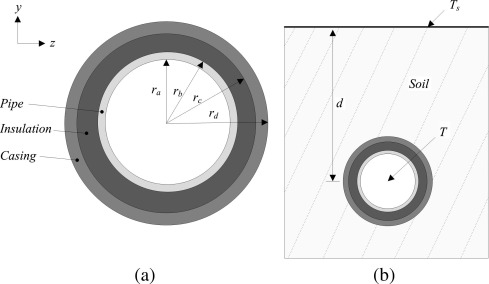
\includegraphics[width=0.5\linewidth]{Literature Survey - DCSC template/figuresLIT/pijpdoorsnede.jpg}
    \caption{Schematic overview of a pipe containing insulation and casing buried in the soil \cite{PipePDE}.}
    \label{fig::pipe}
\end{figure}  

\subsubsection{Modeling Approaches}\label{sec::thermodynamicmethods}
Various methods have been developed to solve the PDE presented in Equation \ref{eq::simpipePDE}. According to the authors of \cite{KUNTUAROVA}, the Node Method is the most widely used approach. Consequently, it has been extensively tested and validated using real-world data. Alternative methods, despite potentially offering greater accuracy or efficiency, have not been subjected to the same level of validation. The Node Method, introduced by Benonysson \cite{BENONYSSON1995297}, calculates the water temperature solely at network node locations, often located at the end of the pipeline. It uses a weighted average of the temperature of the water masses that have entered the pipeline at previous time steps. In \cite{NMvsEM}, the Node Method is compared with the Element Method, which is based on a temperature profile along the pipe. The Node Method turned out to be superior to the Element Method on accuracy and computational cost. It was primarily caused by the problem the Element Method experienced with artificial diffusion (smoothing effect that damps sharp gradients or discontinuities) of the temperature profiles along the pipe. The Node Method experienced the same problem for a Courant Number of around 0.75; this could be easily avoided by choosing a smaller time step. 

In \cite{MAURER2021244}, the authors compare several Finite Difference (FD) approaches to the Node Method. The FD methods approximate the derivatives of the PDE by Difference Quotients (DQ). They only considered the implicit DQ approaches, as the explicit approaches need to fulfill the Courant-Friedrichs-Lewy (CFL) condition, resulting in too many optimization variables because the time step needs to be decreased. It concludes that the Node Method has the smallest computational error with the measurement data for the most discretization steps compared to the FD approaches. Another advantage of the Node Method is that it can handle varying mass flows. However, FD approaches are easier to implement and have a constant number of variables. They also mention an approximation of the Node Method, speeding up the optimization, but only for constant mass flow.

The paper \cite{OPPELT2016336} presents an extension to the Node Method, trying to increase the accuracy of the model by defining the temperature throughout the water masses using a linear interpolation. Van der Heijde et al. \cite{VANDERHEIJDE2017158} validated the model using an experimental pipe setup and demonstrated that it achieves accuracy comparable to the dynamic pipe model in the Modelica Standard Library, while being significantly more computationally efficient. Nevertheless, the Lagrangian method is non-differentiable, making it more difficult to apply for real-time optimization. 

Another method, developed by Zheng et al. \cite{ZHENG2017682}, is known as the Function Method. This approach employs a Fourier series expansion to derive an analytical solution to the transient energy equation. The authors compared it with the Node Method using data from a district heating network in Changchun, China. The Function Method achieved a 37 \% decrease in computation time and notably improved accuracy relative to the Node Method. However, these benefits were observed only under the condition of a constant mass flow rate. 

\subsection{Heat Exchanger}
Heat exchangers are crucial components of the heat distribution system. They exchange thermal energy between the district heating network and the domestic heating system. The Cooltower's heat interface units use plate heat exchangers, which consist of a series of corrugated plates mounted in a frame. Separated by the plates, the hot and cold fluids flow in counter-current or co-current fashion, where they experience a thermal exchange through the thin plate material. 
For this section's modeling approaches it is assumed that the rate of heat transfer from the hot fluid ($\dot{Q_{h}}$, [J / s]) is equal to the rate of heat transfer from the cold fluid ($\dot{Q_{c}}$). That means that we do not lose thermal energy. 

\begin{align}
    \dot{Q_h} &= \dot{m}_hc_h(T_{h,out} - T_{h,in}) = C_h (T_{h,out} - T_{h,in}) \\  
    \dot{Q_c} &= \dot{m}_cc_c(T_{c,out} - T_{c,in}) = C_c (T_{c,out} - T_{c,in})
\end{align}

With the mass flow rates of the hot and cold fluids denoted by \( \dot{m}_h \) and \( \dot{m}_c \) [kg/s], and the specific heat capacities by \( c_h \) and \( c_c \) [J/(kg K)], the inlet and outlet temperatures of the hot fluid are given as \( T_{h,\text{in}} \) and \( T_{h,\text{out}} \) [\( ^\circ \)C], and those of the cold fluid as \( T_{c,\text{in}} \) and \( T_{c,\text{out}} \) [\( ^\circ \)C], respectively. The corresponding heat capacity rates are \( C_h \) and \( C_c \) [J/(K s)] for the hot and cold fluids.

\begin{figure}[htbp]
  \centering
  \begin{minipage}[b]{0.4\textwidth}
    \centering
    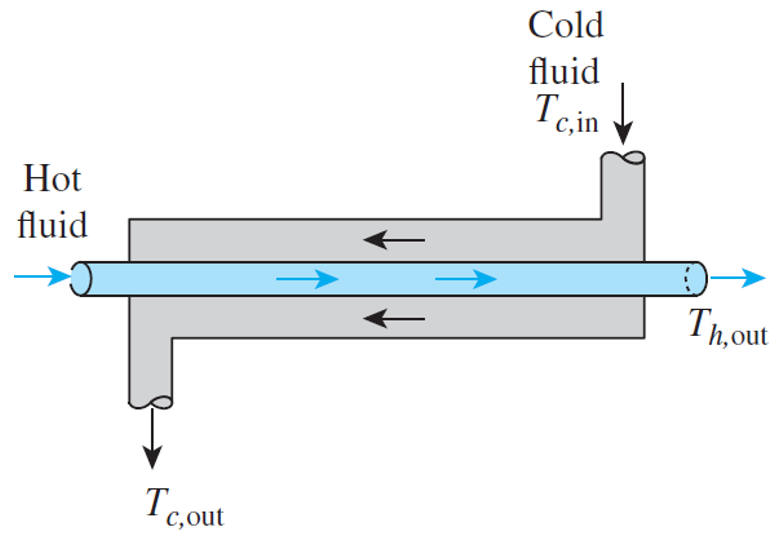
\includegraphics[width=\textwidth]{Literature Survey - DCSC template/figuresLIT/countercurrent.png}
    \caption{Schematic overview of the counter-flow heat exchanger \cite{cengel2025heat}.}
    \label{fig::counterhex}
  \end{minipage}
  % \hfill
  \begin{minipage}[b]{0.4\textwidth}
    \centering
    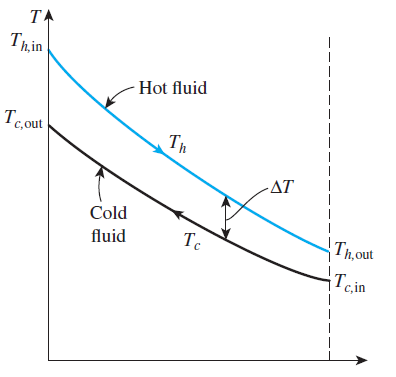
\includegraphics[width=\textwidth]{Literature Survey - DCSC template/figuresLIT/heatexchangerTemperatureprofile.png}
    \caption{Temperature profile along the counter flow heat exchanger \cite{cengel2025heat}.}
    \label{fig::counterflowHEX}
  \end{minipage}
\end{figure}

\subsubsection{Logarithmic Mean Temperature Difference}

Figure \ref{fig::counterhex} shows a basic counter-flow heat exchanger. When there is a difference in heat capacity rates, the temperature difference along the heat exchanger is not consistent, illustrated in Figure \ref{fig::counterflowHEX}. This requires the use of a mean temperature difference ($\Delta T_m$) to be able to use Newton's law of cooling, Equation \ref{eq::newtoncooling}. 
The Logarithmic Mean Temperature Difference ($\Delta_{LM}$) is developed for this case. However, the formula depicted in Equation \ref{eq::LMTD} is determined for the basic counter-flow heat exchanger from Figure \ref{fig::counterhex}, where the plate heat exchanger uses a multi-pass arrangement. To account for this difference in design, a correction factor ($F$) is applied, which is usually around 0.95 for plate heat exchangers \cite{FemkeJanssenLit}. This factor depends on the flow arrangement and the number of transform units (NTU). 

\begin{equation}\label{eq::newtoncooling}
    \dot{Q} =  U A_{s} \Delta T_{m}
\end{equation}
\begin{equation}
    \Delta T_m = F \Delta T_{LM}
\end{equation}
\begin{equation}\label{eq::LMTD}
\Delta T_{\operatorname{lm}}=\frac{(T_{h,in} - T_{c,out}) - (T_{h,out} - T_{c,in})}{\ln \left(\frac{T_{h,in} - T_{c,out}}{T_{h,out} - T_{c,in}}\right)}
\end{equation}
With the overall heat transfer coefficient of the heat exchanger $U$ [J / ($m^2$ K  s)] and the heat transfer surface area $A_{s}$ [m$^2$].

\subsubsection{Effectiveness-NTU method}
In case the outlet temperatures are unknown the Effectiveness-NTU ($\epsilon$-NTU) method can be used. This method revolves around the dimensionless parameter $\epsilon$, the thermodynamic efficiency. 

\begin{equation}\label{eq::epsilon}
    \epsilon = \frac{\dot{Q}}{\dot{Q}_{max}} = \frac{\dot{Q}}{{C}_{min}(T_{h,in} - T_{c,in})}
\end{equation}
\begin{equation}
    C_{min} = \min(C_h, C_c)
\end{equation}
With the thermodynamic maximum achievable power $\dot{Q}_{max}$ [J/s], and the minimum heat capacity rate $C_{min}$ [J/ (K s)]. After performing an energy balance, these values are combined to calculate the heat exchanger effectiveness \cite{cengel2025heat}.
\begin{equation}
    \epsilon = \frac{1 - e^{-NTU  (1 - C^*)}}{1 - C^*  e^{-NTU (1 - C^*)}}
\end{equation}
\begin{equation}
    NTU = \frac{U A_s}{C_{min}}
\end{equation}
\begin{equation}
    C^{*} = \frac{C_{\min}}{C_{\max}}
\end{equation}

\section{Heat supply}
In Section \ref{chap::intro}, it was mentioned that the DCS of the Cooltower is connected to an ATES and a larger district heating network, which serves as a backup during peak demand. In 2024, the heat supplied by this backup network originated primarily from gas boilers (35\%), and excess heat from electricity plants and a waste processing plant (30\% and 16\% respectively) Other contributions came from a biomass power plant (14\%) and residual heat from other sources (5\%) \cite{heatsupply}. 

The ATES dynamics require a complex model as several ground conditions influence heat losses within the aquifers. Additionally, heat losses occur through conduction, advection, and dispersion as the used groundwater is unconfined. Many studies try to capture this by applying the Finite Element Method (FEM) or Finite Volume Method (FVM). \cite{ZHOU2013240,GALGARO2013107,YAPPAROVA20141011}. In a more recent paper, the authors utilized a dynamic mesh optimization, resulting in significantly faster computational time compared to an equivalent fixed mesh while maintaining accuracy \cite{Salinas2022}. System complexity further increases when considering heat/cold injection and extraction integrated with a building or district heating network and coupled with a heat pump. The authors of \cite{BOZKAYA2017620} developed an FEM model and achieved an absolute mean error of less than 0.2 [$^{\circ}\text{C}$] for the wells' temperature. Rostampour et al. \cite{TAMASRostampour} presented a mathematical model for the dynamics of building heating and cooling equipment and ground source heat pump coupled to an ATES, implemented in a model predictive framework. According to \cite{YvoPutter}, buffers can also be approached by a simple discrete state $x(k+1) = \eta_s(x(k) + u_{in}(k)) - u_{out}(k)$, with $\eta_{s}$ as the buffer storage efficiency and $x(k)$ being the level of energy stored at time $k$.  Alternatively, one could completely omit the buffer and assume constant heat or cold injection and extraction, or set it equal to the heat demand. Although it doesn't require a more thorough understanding of the ATES, these simplified approaches might introduce inaccuracies. 

The waste processing plant functions as a combined heat and power (CHP) unit. Sartor et al. \cite{SARTOR2014474} incorporated the dynamics of the CHP system using a quasi steady-state model into their optimization and simulation of a district heating network. Another frequently applied method to replicate its dynamics is the use of Mollier diagrams or Temperature-entropy charts \cite{Laakkonen2017}. These methods provide a better insight into the dynamics of the power production at the cost of a higher computational time. However, as power production can be directly controlled, one can also choose to use a simplified model based on its efficiency and heat generation output. The same holds for the power production of gas boilers and the biomass plant \cite{Talebi,Tamasboilers}. The power coming from excess heat is harder to model. If the necessary data is available, one can choose to apply either a function-fitting or data-driven approach to handle these dynamics. Alternatively, one can simplify the approach by assuming a constant heat output, as the author of \cite{Spruit2020} did for the excess heat of a data center.

Sandou et al.\cite{Sandou2005} chose to use an aggregated model to combine all the power sources of a district heating network and represent it as a quadratic function. They applied a least squares method to find the coefficients. The model was tested on a district heating network benchmark. However, as the production facilities were highly simplified, it is questionable whether this approach would work for this project. More sophisticated predictive time-series methods might be applied, which are discussed in the next Section concerning the heat demand. Eneco holds power production data at a minute-level or more aggregated resolutions, making this type of method a possibility.  


\section{Heat demand}
Heat demand prediction is based on heating demand profiles. These profiles can be tailored for a house, building, or a complete district heating network for various time intervals. The accurate prediction of these profiles influences the network's efficiency and its optimization procedure \cite{ORTIGA20071121}. According to Talebi et al. \cite{Talebi}, heating demand profiles largely consist of three parts: physical and environmental characteristics of the building, occupant behavior, and random factors taking uncertainties into account. They also distinguish three different types of modeling approaches, which are discussed below. 

\subsubsection{Historical Methods}
These methods use historical data from the system's supply and demand to create a demand profile. One approach is to use measurement data as the profile. However, this requires a complete and high-frequency dataset. Eneco collects measurements at the heat interface units of every apartment in the Cooltower. If the user permits sharing the data they can set the data frequency to quarter-hourly, hourly, daily, or monthly. This introduces discrepancies into the data set making direct use of these measurements for the heat profile unlikely. Eneco also has developed their own user heat demand profiles for individual customers with a 15 minute interval. One could also use the Energy Transition Model of Quintel \cite{quintel} that generates the heat demand profile per geographical location based on collected datasets. However, the downside of using such a method is that it provides an average that doesn't take into account real-time parameter values. 

Another method is the use of prototype or archetype buildings. They group buildings in subcategories based on their occupancy. Each category has a reference building from which the demand profiles for the buildings are derived. Lara et al. \cite{ARAMBULALARA2015160} implemented this method using a linear regression model. Other techniques are the Energy Use Intensity (EUI) \cite{sharp1996energy} in combination with the Load Factor (LF) \cite{DALLAROSA20116890}. Where EUI is the rate of energy use per unit area, and LF is the ratio of energy consumption over the maximum possible energy generation of the supply side.

% \todo[inline]{hier aanvullen}
% Heating Degree Day Method and Bin method are other historical methods, but their accuracy is limited due to not including human behavior \cite{ALHOMOUD2001421}.    

\subsubsection{Deterministic Methods}
Deterministic methods are physics-based models. Depending on the approach, the demand profile may be modeled with high detail of the physical behavior of the system or in a simplified form to reduce computational complexity. There are various energy simulation software that can model the thermal behavior of buildings, like Energy Plus \cite{EnergyPlus} and TRNSYS \cite{trnsys1975}. They produce accurate demand profiles, but they come with a big computational cost and require high input data quality \cite{GUADALFAJARA20141096}. The use of simulation software is further discussed in Section \ref{sec::simsoft}. Kim et al. \cite{KIM} applied a simplified method which considered the shape, orientation and occupancy of the building and linearized the dynamics. It achieved an accurate estimate of hourly peak loads with reduced computational time.
 
\subsubsection{Predictive Time-Series Methods}
Predictive time-series methods perform curve fitting to predict the thermal profile of users. One of the common methods is the ARMA model, in which previous demand values are linearly combined with previous and current noise values to predict the user heat demand \cite{GRossGaliana}. Depending on different assumptions relating to the dynamics of the heat demand and the noise, other kinds of ARMA-type models can be used, such as the Box-Jenkins \cite{BoxJenkins}, the ARIMA \cite{ARINA} or SARINA \cite{SARINA}. 

A Finland-based study proposed a day-ahead forecasting approach with a 1-hour interval for various building types, making use of an SVM \cite{SVMFinland}. Neural networks are another machine learning technique widely used in prediction forecasting \cite{ZHANG199835,Hippert,FRISON2024132745}. The Neural networks often outperform other simulation-based methods due to their high adaptability. Although predictive methods achieve a high accuracy, there is a chance of over-fitting and a strong dependence on the quality of the training data \cite{Talebi}.


\section{Simulation Software}\label{sec::simsoft}
Numerous tools exist for simulating energy systems, many of which are also applicable to district heating networks. A lot of the tools are commercial and require a paid license. However, Eneco prefers the use of free simulation software, shifting the main focus of this analysis to free alternatives. Given that Eneco uses Python for internal development, special attention was paid to open-source tools built in or compatible with Python. Nevertheless, to avoid overlooking well-established commercial alternatives, the paid programs WANDA \cite{deltaresWanda} from Deltares, TRNSYS and IDA ICE \cite{IDAICe} were also included in the analysis. WANDA was previously used in a master’s thesis by Femke Janssen on district heating networks \cite{FemkeJanssenLit}, and TRNSYS and IDA ICE are popular simulation tools for energy systems \cite{KUNTUAROVA}. The use of computational fluid dynamics (CFD) programs was briefly considered but deemed too detailed for this project. Table \ref{tab::simsoft} presents a technical comparison of the evaluated tools.

% Please add the following required packages to your document preamble:
% \usepackage{lscape}
\begin{landscape}
\thispagestyle{plain}
\begin{table}[]
% \scriptsize
% \tiny
\fontsize{8pt}{7.5pt}\selectfont
\begin{tabular}{M{3cm}M{3cm}M{1.8cm}M{2.2cm}M{2cm}M{1.5cm}M{2.3cm}M{2cm}p{3cm}}
\hline
Name           & Technical aspects                                            &                      &                  &            &                       &             &                                                                   &                                                                                                                \\ \cline{2-9} 
               & Thermodynamics & Hydraulics    & Optimization\footnotemark[1] & Extendable & Timestep & Components\footnotemark[2] & License                                                           & Remarks:                                                                                                       \\ \hline
DiGriPy \cite{DIGRIPY}  & Static                                                       & Static               & No  & Yes & 1 hour                & 1/1/1/1     & Open source (Python)                                              & Focus specifically on DHN, rarely used                                                                         \\
DHNx \cite{DHNX}          & Static                                                       & Static               & Yes & Yes & 15 min                & 1/0/1/1     & Open source (Python)                                              & Focus specifically on DHN. Some functions only in beta version                                                 \\
EnergyPlan \cite{EnergyPlan}    & Static & Static               & Yes  & Yes & 1 hour                & 0/0/0/0     & Freeware                                                          & Simulation of entire energy systems across all sectors                                                         \\
EnergyPlus \cite{EnergyPlus}     & \makecell{Static, \\ dynamic}                                              & \makecell{\makecell{Static, \\ dynamic}}      & Yes& Yes & 1 min                 & 1/0/1/1     & Open source                                                       & Focus on thermal behavior in buildings and heating systems                                                     \\
Grid Penguin \cite{GridPenguin} & Dynamic                                                      & Static               & Yes & Yes & 1 hour                & 1/0/1/1     & Open source (Python)                                              & Introduced as benchmark, rarely used                                                                           \\
IDA ICE \cite{IDAICe}      & \makecell{Static, \\ dynamic}                                              & \makecell{Static, \\ dynamic}      & Yes & Yes & \textless 1   min\footnotemark[3] & 1/1/1/1     & Commercial, educational                                           & Focus on buildings and HVAC simulation                                                                         \\
OpenModelica \cite{OpenModelica}   & \makecell{Static, \\ dynamic}                                              & \makecell{Static, \\ dynamic}      & Yes & Yes & \textless 1   min\footnotemark[3] & 1/1/1/1     & Open source                                                       & Modelica-based modeling and simulation environment                                                             \\
Pandapipes \cite{pandapipes}     & Static, quasi-static                                         & Static, quasi-static & No & Yes & \textless 1   min\footnotemark[3] & 1/1/1/1     & Open source (Python)  & Focus on multi-energy networks                                                                                 \\
PyDHN \cite{PyDHN}          & Dynamic                                                      & Static               & No & Yes & \textless 1   min\footnotemark[3] & 1/1/1/1     & Open source (Python)  & Currently a beta version.                                                                                      \\
TESPy \cite{TESPy}          & Static                                                       & Static               & Yes & Yes & \textless 1   min\footnotemark[3] & 1/1/1/1     & Open source (Python) & Focus on thermal engineering plants. Also suitable for DHN                                                     \\
TRNSYS \cite{trnsys1975}         & Dynamic (transient)                                          & Dynamic (transient)  & No\footnotemark[4] & Yes & \textless 1   min\footnotemark[3]     & 1/1/1/1     & Commercial, educational                                           & Specializes in building and  HVAC simulations, enabling detailed modeling with an extensive component library. \\
WANDA \cite{deltaresWanda}          & Static                                                       & \makecell{Static, \\ dynamic}      & Yes & Yes & \textless 1   min\footnotemark[3] & 1/1/1/1     & Commercial                                                        & Advanced water hammer software                                                                          
\end{tabular}
\caption{Technical comparison of simulation software of interest.}
\label{tab::simsoft}
\end{table} 
\footnotetext[1]{Only concerning build-in optimization.}
\footnotetext[2]{Pipe/valve/HEX/pump}
\footnotetext[3]{There is no specified minimum timestep, however decreasing it might introduce inaccuracies in the simulation.}
\footnotetext[4]{Optimization possible with TRNOPT.}
\end{landscape}
